\documentclass[10pt]{beamer}

\usetheme{m}

\usepackage{booktabs}
\usepackage{animate}
\usepackage[scale=2]{ccicons}

\title{Deduction as a Service}
\subtitle{}
\date{\today}
\author{Mohamed Bassem}
\institute{German University in Cairo}

\begin{document}

\maketitle

\begin{frame}
  \frametitle{Table of Contents}
  \setbeamertemplate{section in toc}[sections numbered]
  \tableofcontents[
    hideallsubsections,
  ]
\end{frame}

\section{What is E?}
\begin{frame}[fragile]
  \frametitle{What is E?}

  E is a theorem prover that takes a set of axioms and tries to derive a formal proof to a given conjuncture

  \pause{}
  Example:
  \begin{figure}
    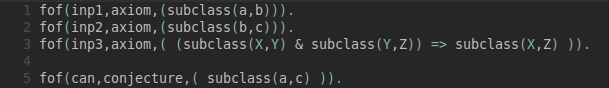
\includegraphics[width=90mm]{imgs/SampleAxioms.png}
  \end{figure}
\end{frame}


\section{Large Axiom Sets}
\begin{frame}[fragile]
  \frametitle{Large Axiom Sets}
  \begin{itemize}[<+- | alert@+>]
    \item OpenCYC library tries to collect the human's common sense knowledge into a comprehensive library with the aim of allowing AI applications to perfom human-like reasoning\cite{wiki:OpenCYC}
      \item Up to 500MB of data and millions of axioms
      \item Other huge axiom sets are extracted from libraries such as SUMO and MIZAR
  \end{itemize}
\end{frame}

\section{Problem}
\begin{frame}[fragile]
  \frametitle{Problem}
  Usually queries only reRunning multiple queries against the same knowledge base requires re-parsing the whole set
\begin{figure} 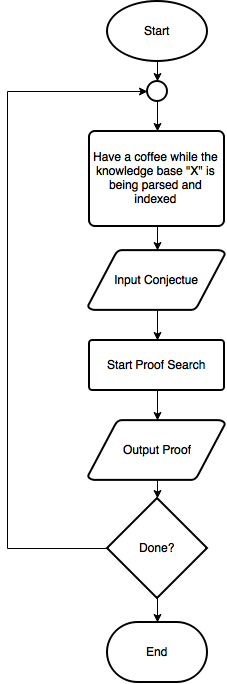
\includegraphics[width=\linewidth,height=0.8\textheight,keepaspectratio]{imgs/OldDeductionFC.png} \end{figure}
\end{frame}


\begin{frame}[fragile]
  \frametitle{Problem}
  No formal way of communicating with E
\end{frame}

\section{Deduction Server}
\begin{frame}[fragile]
  \frametitle{Deduction Server: Sessions}
  \begin{figure} 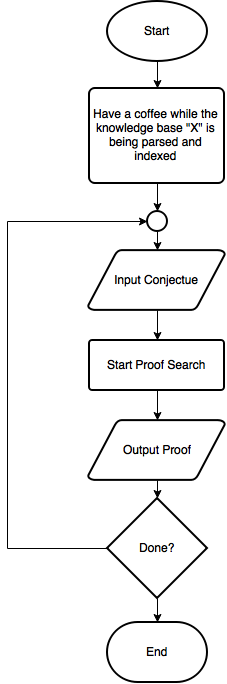
\includegraphics[width=\linewidth,height=0.9\textheight,keepaspectratio]{imgs/NewDeductionFC.png} \end{figure}
\end{frame}

\begin{frame}[fragile]
  \frametitle{Deduction Server: Server Client Architecture }
  \begin{figure} 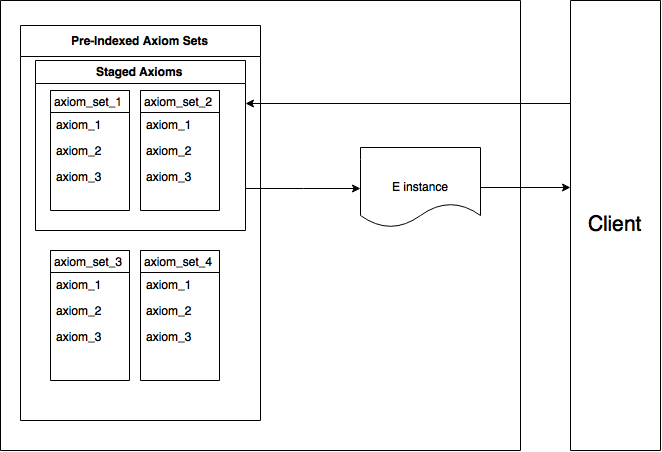
\includegraphics[width=\linewidth,height=\textheight,keepaspectratio]{imgs/TheDeductionServerWithoutPrune.png} \end{figure}
\end{frame}

\begin{frame}[fragile]
  \frametitle{Deduction Server: Pruning}
    \begin{figure} 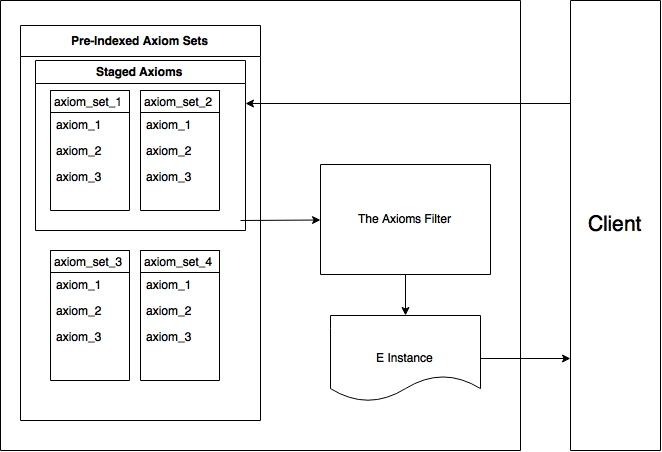
\includegraphics[width=\linewidth,height=\textheight,keepaspectratio]{imgs/TheDeductionServerSingleInstance.png} \end{figure}
\end{frame}

\begin{frame}[fragile]
  \frametitle{Deduction Server: Parallelization}
    \begin{figure} 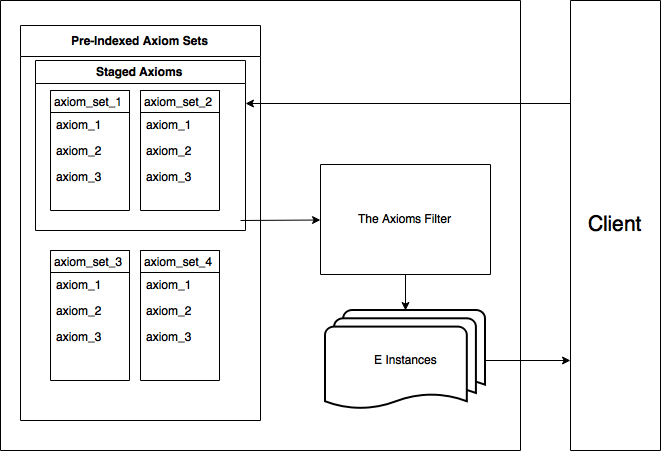
\includegraphics[width=\linewidth,height=\textheight,keepaspectratio]{imgs/TheDeductionServer.png} \end{figure}
\end{frame}

\begin{frame}[fragile]
  \frametitle{Deduction Server: Interaction Protocol}
\end{frame}

\section{Results}
\begin{frame}[fragile]
  \frametitle{Benchmarking}
  \begin{itemize}[<+- | alert@+>]
    \item Tests were performed on a virtualized server with 4 2.6 GHz Intel CPUs with 8 threads
    \item Chosen TPTP Problems:
      \begin{itemize}
        \item 51 Problems
        \item 479 Megabytes on disk
        \item 3,341,984 Formulae
      \end{itemize}
    \item Test Setup:
      \begin{itemize}
        \item The deduction server ran in the single strategy mode using the same strategy as the plain eprover
        \item Time Limit: 30 Seconds
        \item Memory Limit: 1024 MB
      \end{itemize}
    \item Time was recorded after 5, 10, 20, 30, 40 and all 51 problems
  \end{itemize}
\end{frame}


\begin{frame}[fragile]
  \frametitle{Benchmarking}
\begin{figure} 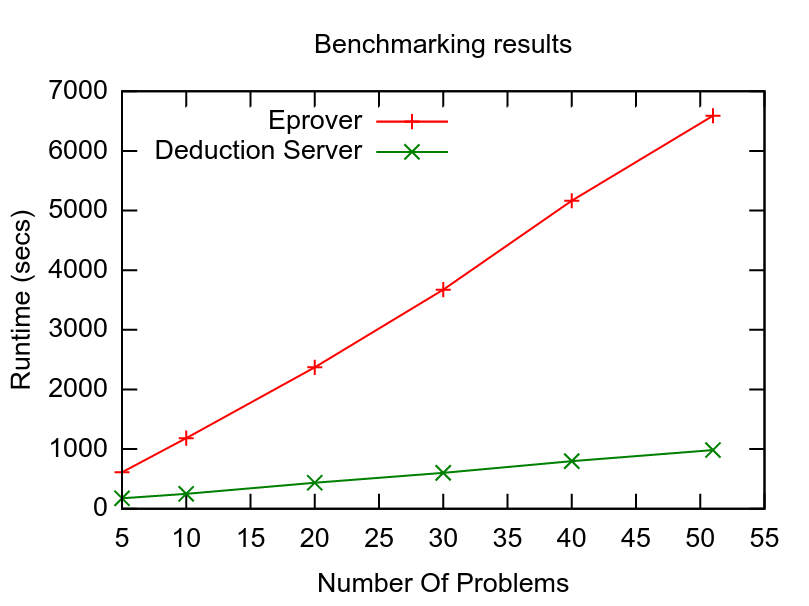
\includegraphics[width=\linewidth,height=0.9\textheight,keepaspectratio]{imgs/BenchmarkingResults.png} \end{figure}
\end{frame}

\begin{frame}[fragile]
  \frametitle{Deduction as a Service}
  \begin{itemize}[<+- | alert@+>]
    \item Having a hosted deduction server will allow users to connect to the remote server and have their own sessions
    \item A win for:
      \begin{itemize}
          \item Users who cannot install the prover due to compatiblity issues
          \item Users who have limited resources
      \end{itemize}
    \item Before The protocol, apps used to interacting with E by invoking the executable in a subprocess. The interaction protocl will make it much easier to intgerate apps with E
  \end{itemize}

\end{frame}

\section{Future Work}
\begin{frame}[fragile]
  \frametitle{Future Work}
  \begin{itemize}[<+- | alert@+>]
    \item Controlling client allowed resource
    \item Clustering and load balancing
    \item Supporting other backends
    \item Supporting other pruning techniques
  \end{itemize}
\end{frame}

\section{Conclusion}
\begin{frame}[fragile]
  \begin{itemize}[<+- | alert@+>]
    \item Benchmarking results shows that the deduction server mode outperforms plain eprover in large axiom sets with shared knowledge bases
    \item Offering deduction as a hosted service will allow users to use remote theorem provers on powerful servers
    \item The interaction protocol makes integrating apps with E much easier
  \end{itemize}
\end{frame}

\plain{Questions?}
\plain{Thank you}

\begin{frame}[allowframebreaks]

  \frametitle{References}

  \bibliography{presentation}
  \bibliographystyle{abbrv}

\end{frame}

\end{document}
